\chapter{Thermal flow in curved pipe}

\modinfo{Files}{curved\_pipe.grd}
\modinfo{Solvers}{\Idx{HeatSolve}, \Idx{FlowSolve}}
\modinfo{Tools}{\Idx{ElmerGUI}}
\modinfo{Dimensions}{3D, Steady-state}
\modinfo{Author}{Peter R{\aa}back}


\subsection*{Case definition}
 
%\begin{flushleft}

This tutorial demonstrates how to set up a coupled case
of thermal flow in curved pipe with a finite thickness. Within the pipe 
both the flow and heat transfer equations need to be solved while on the
solid section only heat transfer needs to be considered. 

The inner diameter of the pipe is 0.01~m and the outer ~0.012~m, respectively. 
It is bent to a 135 degree angle with a radius of 0.02~m. Beyond the bend
0.03~m of the direct part is also accounted for. 
The fluid flowing in the pipe is water with an original temperature of 350~K. 
The outer temperature of the iron pipe is 300~K making the water
gradually to cool. 

The water is injected with a parabolic velocity profile with a maximum
of 0.01~m/s. In reality the laminar analytic profile is described by the 
Bessel's function. Here the flow is treated as laminar and steady-state 
even though at these Reynolds number (about 100) the unsteady nature of the 
flow should probably be considered. This would enhance the heat transfer.
The steady-state case, however, will achieve the educational goals of the tutorial.

\subsection*{Solution procedure}

The mesh is defined in ElmerGrid format in file \texttt{curved\_pipe.grd}, load this file.
\ttbegin
File 
  Open -> curved\_pipe.grd
\ttend
You should obtain your mesh and may check that it consists of 23670 trilinear 
bricks and 25245 nodes. The density of the mesh may be varied by altering
the \texttt{Reference Density} in the file. For further information on
the mesh definition look at the \texttt{ElmerGrid} manual. Often it is 
desirable to use some professional mesh generation tool in CFD and 
translate it into Elmer format. For educational purposes we are 
quite happy to use this simple geometry.  

\begin{figure}[h]
\centering
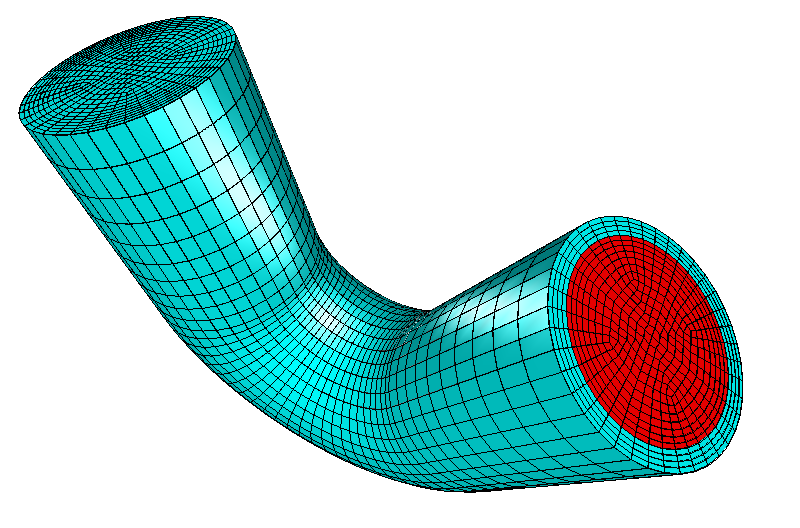
\includegraphics[width=10cm]{curved_pipe_gui}
\caption{The mesh of the curved pipe as seen in ElmerGUI}\label{fg:curved_pipe_mesh}
\end{figure} 


After we have the mesh we start to go through the \texttt{Model} menu from the top to bottom. 
In the \texttt{Setup} we choose things related to the whole simulation such as file names, 
time stepping, constants etc.
The simulation is carried out in 3-dimensional Cartesian
coordinates in steady-state. There is nothing really to be done here, but you may verify that
the defaults are correct. 
\ttbegin
Model
  Setup 
    Coordinate system = Cartesian
    Simulation type = Steady state
    Steady state max. iter = 1
    ...
\ttend

In the Equation section we choose the relevant equations and parameters related to their solution. 
In this case we'll have two different sets of solvers (called as Equation in Elmer slang). 
The other consists of heat and flow solvers, while the 
other includes just the heat solver. We'll name them appropriately. 

When defining Equations and Materials it is possible to assign to the bodies immediately, or to use mouse
selection to assign them later. In this case we know that the fluid body has the index 1 and the 
solid body has the index 2. Therefore it is easy to assign the Equation and Material to the bodies directly. 

Here we neglect the effect of natural convection. Therefore there is just one-directional coupling from the 
flow to heat transfer. In order to follow the direction of causality we address the flow solver with a higher 
priority than the heat solver (default is zero). 	

Here we are quite happy with the default solver settings of the individual equations. 
However, for the flow solver we change the default proconditioner \texttt{ILU0} to \texttt{ILU1} to 
enhance convergence (with increased memory consumption). For 3D cases the direct solvers are usually 
not feasible so it is better to stick with the iterative \texttt{BiCGstab} linear solver. 
\\
The equation for the fluid
\ttbegin
Model
  Equation
    Add
    Name = Heat and Flow
    Apply to Bodies = 1
    Heat Equation
      Active = on
      Convection = Computed
    Navier-Stokes 
      Active = on
      Priority = 1
      Edit Solver Setting
        Linear System
          Preconditioning = ILU1
    OK
\ttend        
and then for the solid
\ttbegin
Model
  Equation
    Add
    Name = Just Heat
    Apply to Bodies = 2
    Heat Equation
      Active = on
      Convection = None
    OK
\ttend    


The Material section includes all the material parameters.
They are divided into generic parameters which are direct properties of the material
without making any assumptions on the physical model, such as the density. Other properties assume
a physical law, such as conductivities and viscosity. 

Here we choose water and iron from the material library.
You may click trough the material parameters of the various solvers to ensure that
the properties are indeed as they should be. Any consistent set of units may be used in Elmer.
The natural choice is of course to perform the computations in SI units. 

\ttbegin
Model
  Material
    Add
    Material library    
      Water (room temperature)
    Apply to Bodies = 1 
    OK

    Add
    Material library    
      Iron (generic)
    Apply to Bodies = 2
    OK
\ttend

The \texttt{Body force} section usually represents the right-hand-side of an equation. It could be used to account for the 
natural convection, for example. In this case, however, we do not apply any body forces.

Also an \texttt{Initial condition} could be given in steady-state case to enhance convergence. However, 
in this case convergence is pretty robust with the default guess of zero.

We have four different boundary conditions: thermal inflow, internal no-slip, 
outflow, and external fixed temperature. Otherwise natural BCs are assumed.
As it is tedious to know the indexes by heart we 
first define the different BCs and only afterwards apply them to the existing boundaries 
with the mouse. 

\ttbegin
Model
  BoundaryCondition
    Name = HotInflow
    Heat Equation
      Temperature = 350.0
    Navier-Stokes 
      Velocity 1 = 0.0
      Velocity 2 = 0.0
      Velocity 3 = Variable Coordinate 
        Real MATC "100.0*(1.0e-4-tx(0)^2-tx(1)^2)"
    Add
    New
\ttend
The condition for \texttt{Velocity 3} above may easiest be typed by pressing \texttt{Enter}-key in the
edit box which will open a larger window for editing.
\ttbegin
    Name = Outflow
    Navier-Stokes 
      Use normal-tangential coordinate system = on
      Velocity 2 = 0.0
      Velocity 3 = 0.0
    Add
    New

    Name = NoSlip
    Navier-Stokes 
      NoSlip Wall BC = on
    Add 
    New
 
    Name = Troom
    Heat Equation
      Temperature = 300.0
    Add
\ttend   

When choosing the boundaries it is important that you choose the right inlet.
For that purpose you may activate the compass, 
\ttbegin
View
  Compass = on
\ttend
Now the inlet is the one with normal pointing at the $z$-direction.
Now we are ready to choose the boundaries 
\ttbegin
Model
  Set boundary properties
    Choose inlet face -> set boundary condition HotInflow
    Choose outlet face -> set boundary condition Outflow
    Choose outer side -> set boundary condition Troom
\ttend
Unfortunately we cannot see the internal boundary. For that purpose click on the 
outer boundary and choose 
\ttbegin
View
  Hide/show selected
\ttend
The outer boundary should vanish and you can
proceed with the last BC,
\ttbegin
Model
  Set boundary properties
    Choose internal side -> set boundary condition Noslip
\ttend


For the execution 
ElmerSolver needs the mesh files and the command file. We have now basically defined
all the information for ElmerGUI to write the command file. After writing it we may also visually 
inspect the command file.
\ttbegin
Sif 
  Generate
  Edit -> look how your command file came out  
\ttend

Before we can execute the solver we should save the files in a directory. The project includes
all the files needed to restart the case. It's a good idea to give the project an illuminating name.
Avoid paths which includes empty spaces since they may cause problems later on. 
\ttbegin
File 
  Save Project
    Make New Folder -> curved_pipe
    OK
\ttend

After we have successfully saved the files we may start the solver
\ttbegin
Run
  Start solver
\ttend
A convergence view automatically pops up showing relative changes of each iteration.
The simulation may take a few minutes depending on your platform. 
After the simulation has terminated we may study the results.
\begin{figure}[h]
\centering
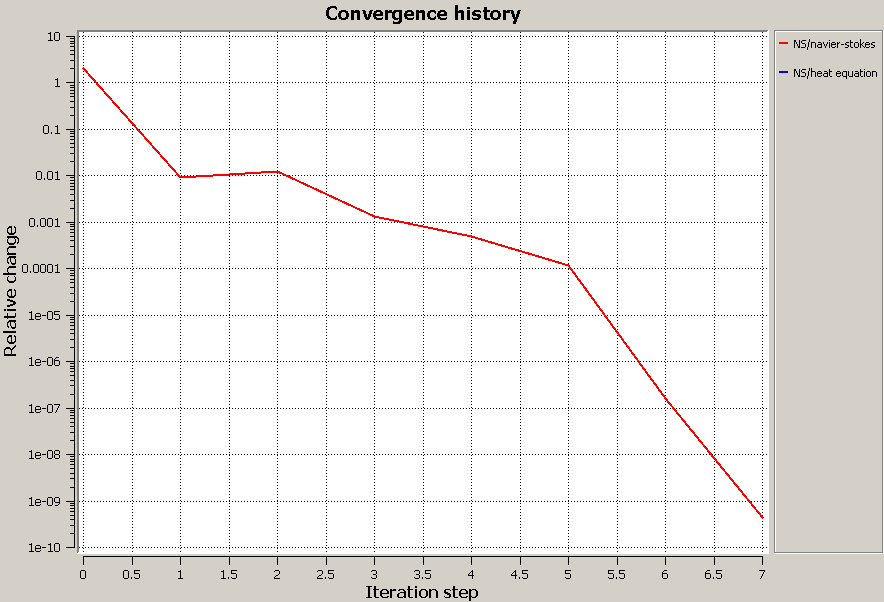
\includegraphics[width=10cm]{curved_pipe_convergence}
\caption{Convergence history of the case}\label{fg:curved_pipe_convergence}
\end{figure} 

\subsection*{Results}

The computed norms should be 3.255 for the Navier-Stokes equation and
324.66 for the heat equation. If there is some discrepancy the setup of the system
was probably different from the one in the tutorial.

After the simulation has terminated we may open the postprocessor to view the results.
\ttbegin
Run
  Start ParaView
\ttend

A standard way of visualizing is to choose \texttt{ColorMesh} and 
there choose \texttt{Surface} and the desired field variable, for example 
\texttt{Velocity\_abs} or \texttt{Temperature}. In this case only the 
outflow cross section contains any information. It may be seen in 
Figure~\ref{fg:curved_pipe_temp_end} that the symmetry around pipe origin is lost in the 
bend. 
\begin{figure}[h]
\centering
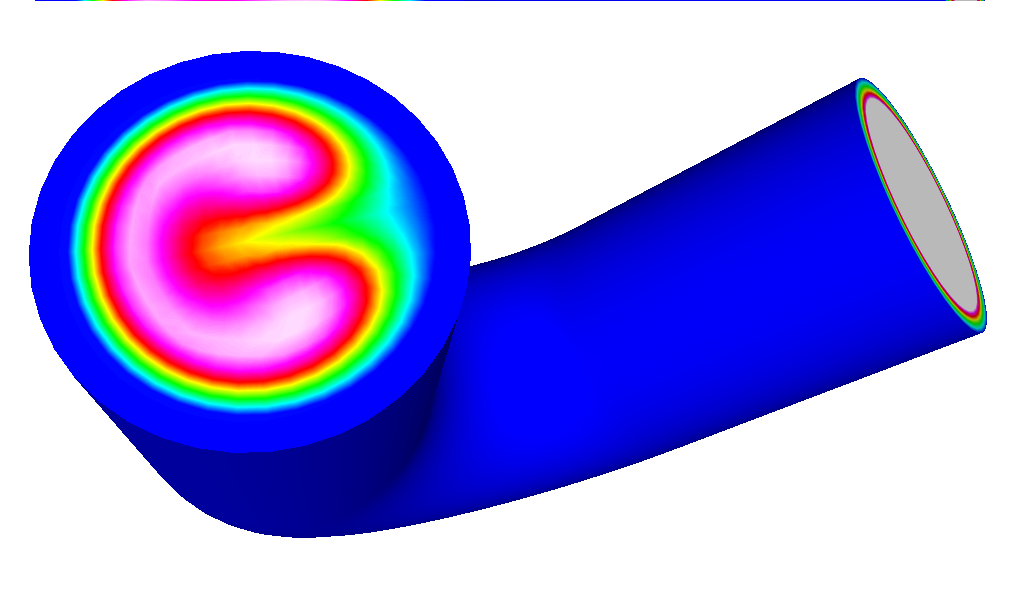
\includegraphics[width=8cm, viewport=0 20 1024 580,clip]{curved_pipe_velo_end}
\caption{Temperature distribution at the outlet of the pipe}\label{fg:curved_pipe_temp_end}
\end{figure} 

Alternatively we may visualize the cross section at $y=0$. To that aim choose 
\texttt{Isocontours} and there set the \texttt{Number Of Isosurfaces} to 1, 
choose \texttt{Surface}, set \texttt{Contour Variable} to \texttt{nodes\_y}, and 
\texttt{Color Variable} to \texttt{Temperature} etc. Now you may nicely see how the 
velocity profile affects the temperature distribution in the pipe.

In Figures \ref{fg:curved_pipe_temp} and \ref{fg:curved_pipe_velo} the obtained velocity and temperature 
distributions are presented. 

\begin{figure}[h]
\centering
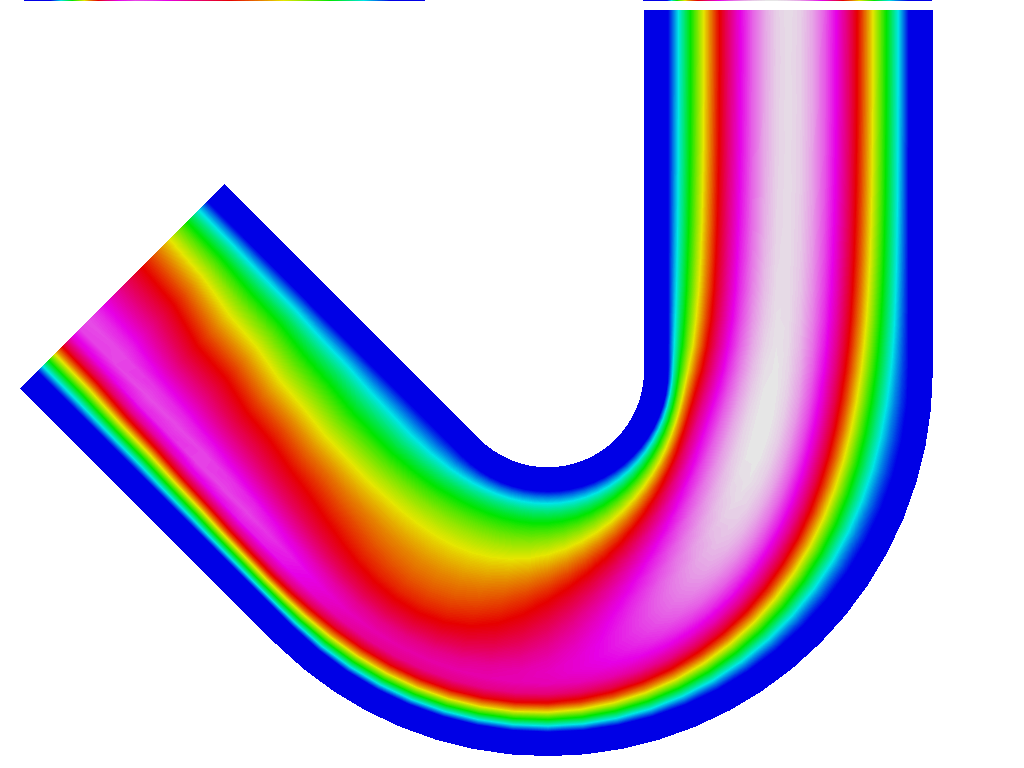
\includegraphics[width=10cm, viewport=0 8 1024 750,clip]{curved_pipe_velo_crosssection}
\caption{Velocity distribution at the cross section $y=0$.}\label{fg:curved_pipe_velo}
\end{figure} 

\begin{figure}[h]
\centering
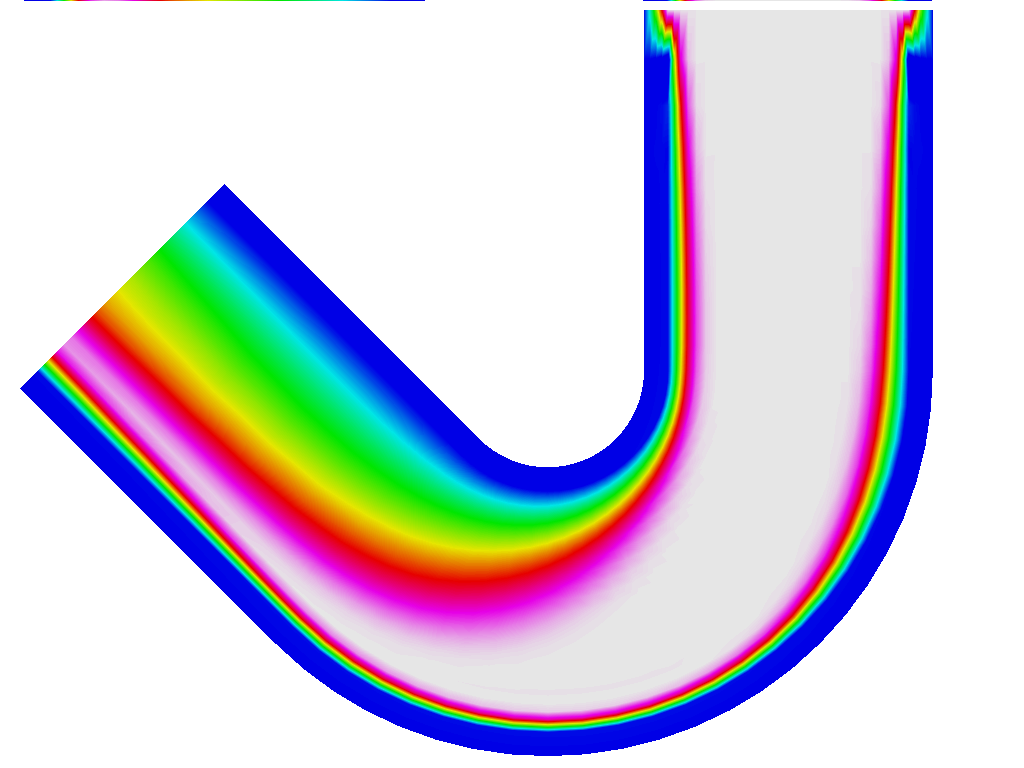
\includegraphics[width=10cm, viewport=0 8 1024 750,clip]{curved_pipe_temp_crosssection}
\caption{Temperature distribution at the cross section $y=0$.}\label{fg:curved_pipe_temp}
\end{figure} 



\hfill
